\documentclass{article}
\usepackage{graphicx}
\usepackage{url}
\usepackage{minted}
\usepackage{url}

\bibliography{rapport.bib}{}
\newcommand\thickbar[1]{\accentset{\rule{.4em}{.8pt}}{#1}}

\title{Adversarial Models: Computer Security Issues}
\author{Auriane Blarre, Romain Kakko-Chiloff and Louis R\'emus}
\date{November $3^{rd}$,  2017}

\begin{document}
\maketitle

\section{Introduction}
A growing ensemble of tasks is being delegated to machine learning algorithms. Among them, classification of images is a major subset, especially with the recent developments of self-driving technology. Recent studies by Google Brain have shown that any machine learning classifier can be tricked to give incorrect predictions. Indeed, it is possible to trick them to get results very different from what is expected, and sometimes, pretty much any result you want.
\newline
We can understand why these results are worrisome: imagine that you could fool an ATM machine and cash a check of \$1,000,000 instead of \$1,000, or fool a self-driving car with a phony stop sign interpreted by the device as a speed limit increase to 200.
As our world relies more and more on automated classifiers, it is crucial to understand their limitations and the way wrongdoers could exploit them.

\section{Project Outline}
\subsection{Problem description}
Adversary attacks "trick" machine learning algorithms into making a wrong prediction by adding specific noise to the input data. The term noise here is not really appropriate, since the perturbation is intended and oriented so as to exploit the model's flaws.
\newline
There are two types of attacks:

\begin{itemize}
    \item Non-targeted attacks simply aim at making the algorithm make an erroneous prediction
    \item Targeted attacks want the algorithm to make a specific prediction
\end{itemize}

% Adversarial example car figure
\begin{figure}[ht]
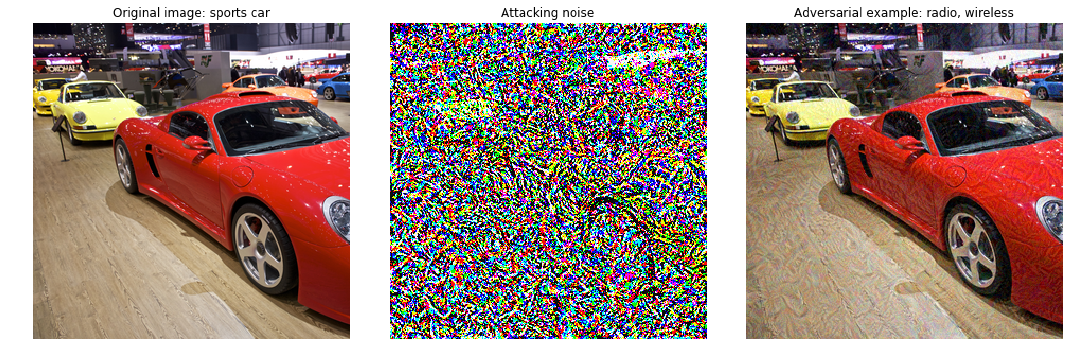
\includegraphics[width=\textwidth]{fig/adversarial_example_car.png}
\centering
\caption{Example of an adversarial attack}
\end{figure}

\newpage
\subsection{Our scope}
We will focus on the problem of image classification.
We aim at:

\begin{itemize}
    \item Implementing different classification algorithms to tag our image set with a decent accuracy
    \item Finding out for each algorithm a distribution of "noise" not perceptible by the naked eye that would trick the algorithm into making a wrong prediction, in the two cases aforementioned:
    \begin{itemize}
        \item Non-targeted attacks
        \item Targeted attacks
    \end{itemize}
\end{itemize}

We will then compare how robust the algorithms are with regards to these two types of attacks. We will also rate how easy each algorithm is to attack as a function of its parameters. For instance, we will pay special attention to the bias-variance trade-off: does increasing bias make an algorithm more robust? Intuitively, a very biased algorithm will be easy to trick in a non-targeted fashion, but harder in a targeted-fashion.
\subsection{Models}
We plan on testing the following models:

\begin{itemize}
    \item Neural Networks (Inception)
    \item Support Vector Machines
\end{itemize}

\subsection{Data}
We plan on using the dataset of images provided by Google Brain for the Kaggle challenge "NIPS 2017: Adversarial Learning Development" \cite{a2}.

\subsection{Tools}
We will use the common Python libraries \texttt{scikit-learn} and \texttt{tensorflow} \cite{tensorflow}. We will also use the building tool \texttt{travis} and the checker \texttt{pylint} to ensure a clean and modularized code.

\subsection{Possible developments}
Can we detect the presence of an adversarial example?
This is a apparently hard question that we would like to explore. Assume the image is the one of a toaster. If the attack is not subtle and the "noise" visible, a human agent easily identifies the attack: he notices the colored "noise" on the toaster image. But for our model, the image \textbf{is} the one of, say, a whale. The model might even be so sure about it that it will not question its own decision and report a suspicious sample to another program.

We would like to try methods and train models so as to be able to identify whether a suspicious "noise" was added to the original image. In short, "noise" with a certain shape that would make highly doubtful.

\section{Timeline}

As the project lasts only one month, we will have to deploy an efficient methodology. We have decided to work with weekly objectives as it is mentioned in the following :
\begin{itemize}
    \item Week 1 : Model benchmarking and first adversarial experiments
    \item Week 2 : Bias-variance trade-off
    \item Week 3 : Development of a model to detect adversarial inputs
    \item Week 4 : Finalization of the results
\end{itemize}



\begin{thebibliography}{1}

    \bibitem{a1} Emil Mikhailov; Roman Trusov {\em How Adversarial Attacks Work} 
  "\url{http://blog.ycombinator.com/how-adversarial-attacks-work/}"
  
    \bibitem{a2} Google Brain {\em NIPS 2017: Adversarial Learning Challenges} 
    \newline
    \url{https://www.kaggle.com/benhamner/adversarial-learning-challenges-getting-started}
    
    \bibitem{tensorflow}
    The Tensorflow authors.
    \url{https://www.tensorflow.org/}.

  \end{thebibliography}

\listoffigures

\end{document}